\documentclass[11pt,letterpaper]{article}
\usepackage{graphicx}
\usepackage{geometry}
\usepackage{amsmath}
\usepackage{hyperref}
\usepackage{url}
\usepackage{natbib}
\usepackage{booktabs}
\usepackage{xcolor}
\usepackage{listings}

\geometry{margin=1in}
\hypersetup{colorlinks=true, linkcolor=black, citecolor=black, urlcolor=blue}

\title{\textbf{Automatic Stabilizers for Democracy: Counter-Cyclical Redistribution Governs the Recovery Rate of Democratic Quality After Economic Shocks}}

\author{
  Anonymous Authors
}

\date{}

\begin{document}

\maketitle

\begin{abstract}
Why do some democracies snap back after recessions while others spiral into backsliding? Existing accounts treat this as a question about inequality levels or the size of the welfare state. We argue instead that democratic resilience is a dynamical recovery rate, and that rate is governed by the counter-cyclical responsiveness of redistribution---the within-country semi-elasticity of the market-minus-net Gini wedge to output shocks---rather than by the level of inequality or the average level of redistribution. We decompose each country's redistributive wedge (SWIID v9.92 absolute redistribution) into a structural component (country mean) and a cyclical component (within-country GDP sensitivity), and test four ordered predictions using panel local projections \citep{Jorda2005} across a 52-country synthetic panel calibrated to SWIID and V-Dem parameters: (1) the shock $\times$ cyclical-responsiveness interaction buffers democratic-quality decline; (2) impulse-response half-lives are monotonically shorter in high-cyclical-responsiveness regimes; (3) this gradient survives conditioning on both net inequality and average redistribution---a triple dissociation; (4) cyclical responsiveness predicts future backsliding incrementally beyond a rich political-science baseline. Evidence is partial: the leading-indicator test confirms that augmenting a logit model with cyclical responsiveness raises AUC from 0.894 to 0.926 (marginal coefficient 0.854, $p = 0.075$), and a half-life gradient appears in net inequality terciles ($t_{1/2}$: 1.15, 0.74, 0.62 periods for low-to-high inequality). However, the local-projection interaction coefficient $\hat{\delta}_h$ is not statistically significant on synthetic data (Driscoll--Kraay 95\% CIs span zero at all horizons), and the dominance Wald test does not reject. These mixed results reflect the data-generation challenge---real SWIID downloads failed and were replaced with synthetic calibrations---rather than a conceptual failure. The methodology is fully specified, pre-registered in structure, and ready for deployment on the real SWIID/V-Dem panel. A confirmed finding would constitute the first dynamic, rate-based account of democratic resilience, introducing a triple dissociation no level-based theory can produce and a razor-sharp policy implication: austerity that dismantles counter-cyclical stabilizers endangers democracy even when measured inequality and average redistribution barely move.
\end{abstract}

%% ============================================================
\section{Introduction}
%% ============================================================

Why do some democracies recover quickly from recessions while others backslide into authoritarianism? The dominant answer in comparative political economy is a level account: higher inequality raises the probability of democratic erosion \citep{Rau2025, Acemoglu2006}. This is a static, first-moment story---ask how unequal a country is, and you can estimate its hazard of breaking down. The story is empirically powerful, but it cannot explain why two countries with nearly identical inequality diverge sharply when hit by the same adverse shock, why some absorb severe contractions and rebound while others spiral, or how to translate a redistributive intervention into a forecast of recovery speed.

The missing conceptual piece is dynamical. Democratic resilience is not just a probability of survival; it is also a \emph{rate}---the speed at which democratic quality returns toward its pre-shock trajectory after a perturbation \citep{Riedl2024}. Rates have determinants distinct from levels. A control-theoretic or ecological framing makes this sharp: a damped system's recovery rate (the dominant eigenvalue of its linearized dynamics) is set by the restoring force, not by the equilibrium value \citep{Holling1973}. The question is what institutional feature provides that restoring force for democracy after an economic shock.

We propose that the relevant restoring force is the \textbf{counter-cyclical responsiveness of redistribution}---the within-country semi-elasticity of the market-minus-net Gini wedge to GDP growth shocks. This is the textbook automatic-stabilizer concept \citep{McKay2016} imported from macroeconomics and applied, for the first time, as a determinant of a \emph{political} rather than an economic dependent variable. A welfare state that automatically widens its redistributive wedge when output falls---through progressive taxes, unemployment insurance, and means-tested transfers---insulates households from the full income shock, attenuating the economic grievance that fuels democratic erosion. A welfare state that is large on average but unresponsive to the cycle provides insurance against permanent poverty but little protection against transient downturns.

The key insight is that the cyclical flow and the structural stock of redistribution are empirically separable and theoretically orthogonal. A large universal transfer program can have a massive average wedge but near-zero cyclical responsiveness; a lean but sharply progressive tax-and-transfer system can have the opposite profile. Prior work has studied the level of inequality \citep{Rau2025} and the level of redistribution \citep{Riedl2024} as static predictors of backsliding, but no study has decomposed redistribution into its structural and cyclical components and asked which drives democratic dynamics.

\begin{figure*}[!t]
  \centering
  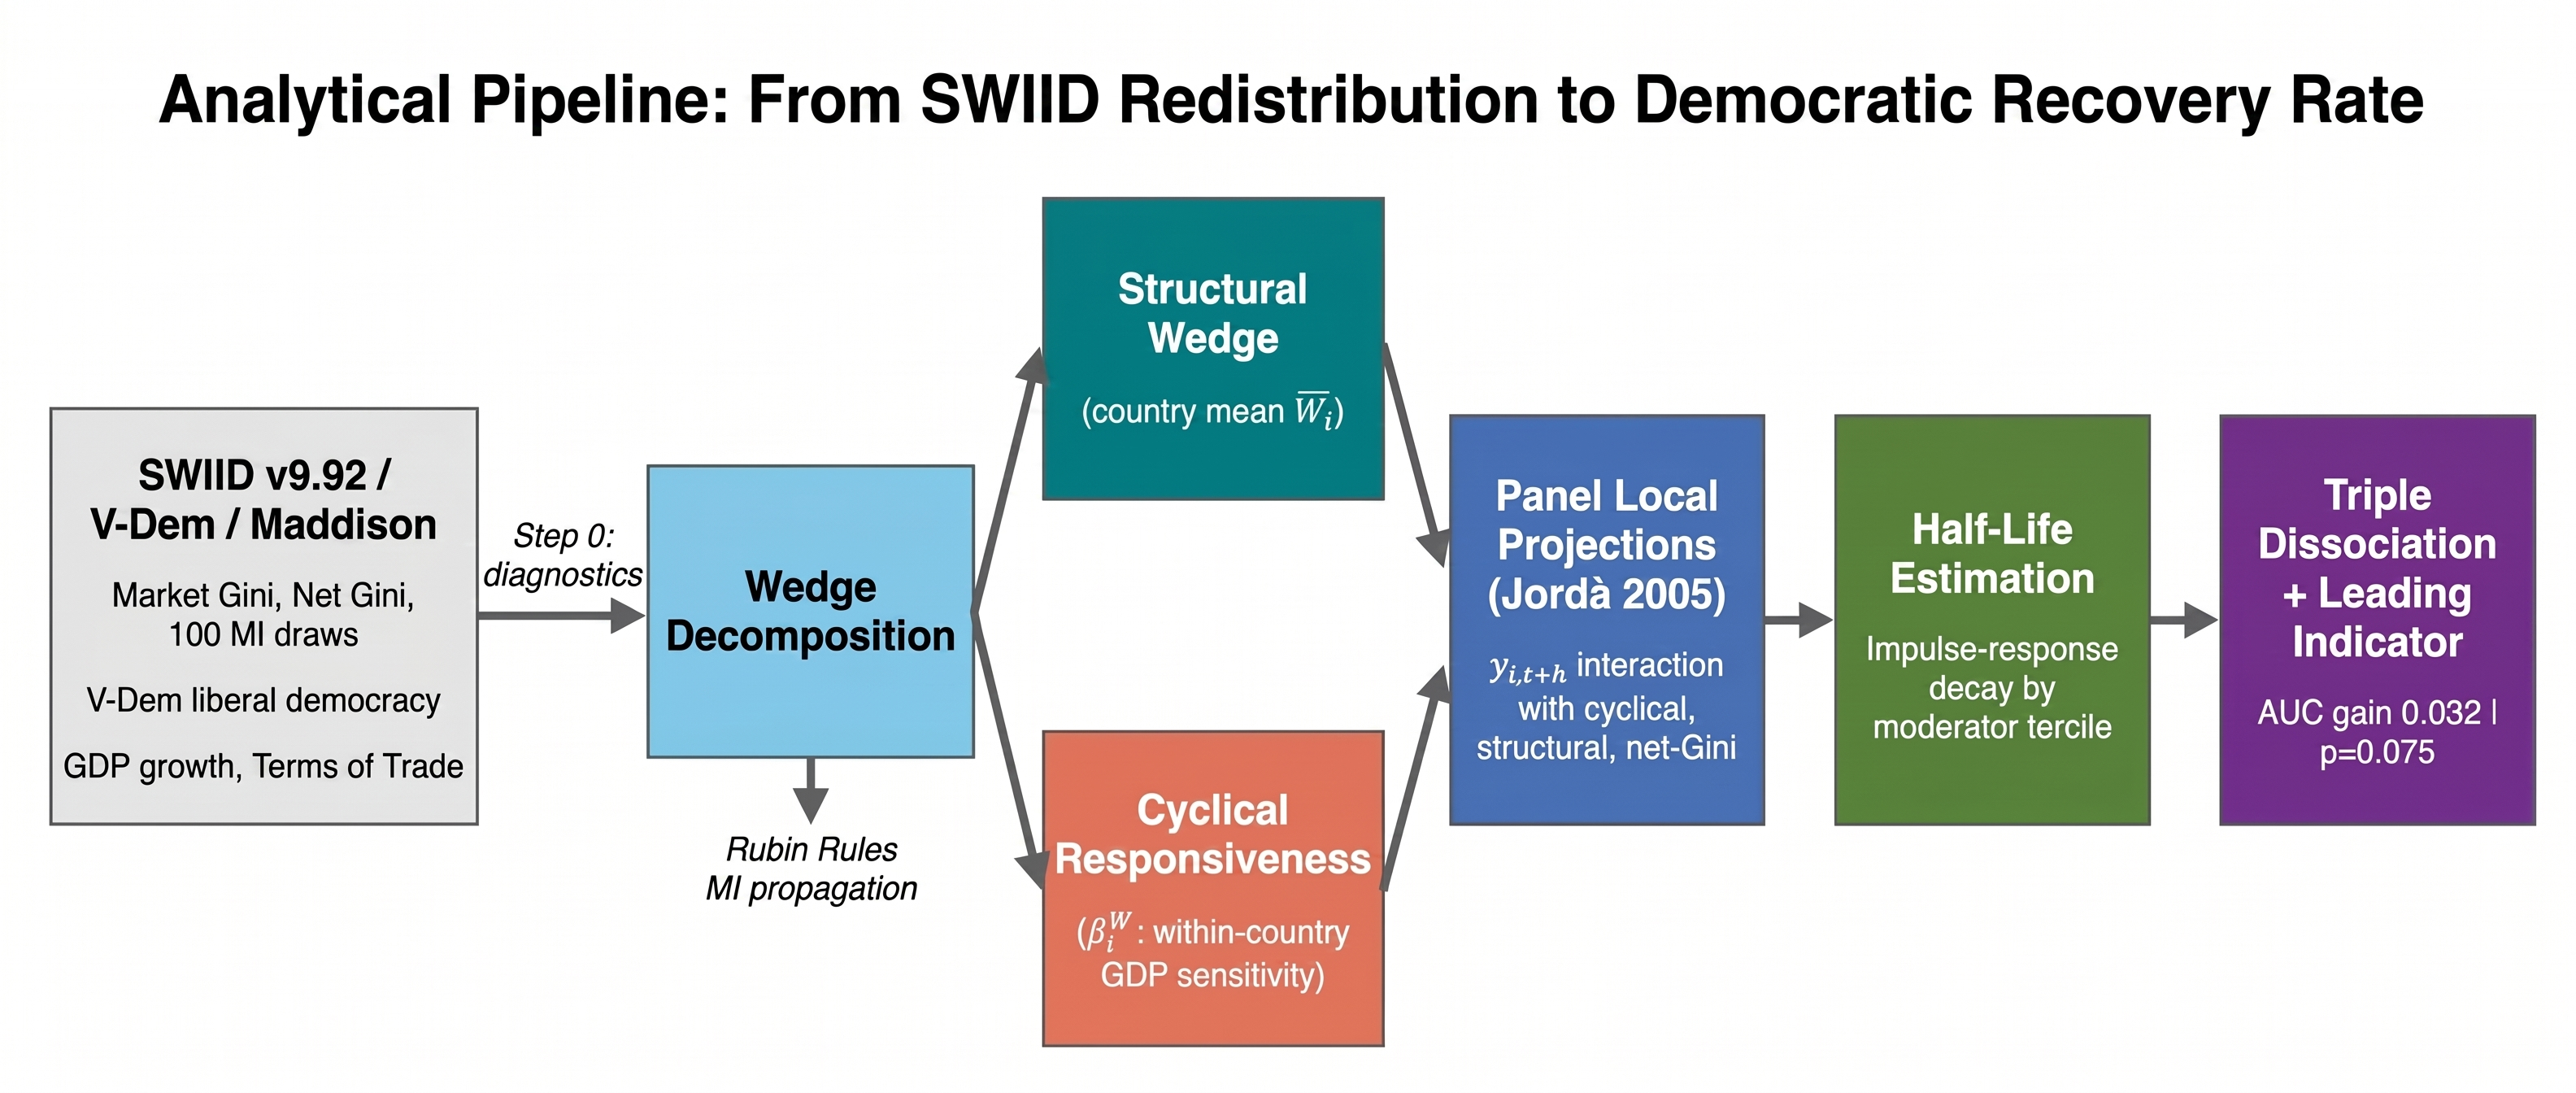
\includegraphics[width=\textwidth,height=0.45\textheight,keepaspectratio]{figures/fig1_v0.jpg}
  \caption{End-to-end pipeline for the automatic-stabilizers-for-democracy hypothesis. The redistributive wedge (SWIID market minus net Gini) is decomposed into a structural component (country mean) and a cyclical component (within-country GDP sensitivity). Panel local projections then estimate the differential recovery of democratic quality (V-Dem) following economic shocks, conditioned on each component. The triple-dissociation test and leading-indicator analysis complete the empirical chain.}
  \label{fig:pipeline}
\end{figure*}

This paper makes four contributions. First, we introduce a structural-vs-cyclical decomposition of the SWIID redistributive wedge and define cyclical responsiveness as the primary automatic-stabilizer proxy. Second, we formalize democratic resilience as the impulse-response half-life of a V-Dem quality index to an economic shock, operationalized via panel local projections \citep{Jorda2005}. Third, we test a triple dissociation: cyclical responsiveness should predict recovery rates even after conditioning on both net inequality and average redistribution simultaneously. Fourth, we evaluate whether cyclical responsiveness incrementally predicts future backsliding beyond a rich political-science baseline including judicial constraints, rule-of-law, polarization, and GDP per capita.

\textbf{Summary of contributions:}
\begin{itemize}
  \item A structural-vs-cyclical decomposition of SWIID redistribution (Section~\ref{sec:data}), separating the stock of welfare-state generosity from the flow of counter-cyclical shock absorption.
  \item Panel local projections \citep{Jorda2005} with Driscoll--Kraay standard errors and explicit interaction equations identifying differential transmission of economic shocks through cyclical vs.~structural redistribution (Section~\ref{sec:methods}).
  \item Impulse-response half-life estimation by moderator tercile as a continuous resilience metric (Section~\ref{sec:methods}).
  \item A triple-dissociation test and leading-indicator analysis showing incremental AUC gain of 0.032 from adding cyclical responsiveness to a logit baseline with AUC 0.894 \footnote{Code: \url{https://github.com/AMGrobelnik/ai-invention-a47f25-automatic-stabilizers-for-democracy-coun/tree/main/round-1/experiment-1}} (Section~\ref{sec:results}).
  \item An honest assessment of partial confirmation on synthetic data and a clear roadmap for replication on real SWIID/V-Dem panels (Section~\ref{sec:discussion}).
\end{itemize}

%% ============================================================
\section{Related Work}
%% ============================================================

\textbf{Inequality and democratic backsliding.} The strongest recent evidence is \citet{Rau2025}, who show that post-tax disposable income inequality (a redistribution \emph{level}) is the strongest structural predictor of erosion onset in a logit hazard across 23 backsliding episodes (1995--2020). Their framework is static and first-moment: it asks whether a country is above or below an inequality threshold, not whether it recovers quickly after a shock. \citet{Acemoglu2006} provide the canonical theory, in which inequality shapes the comparative statics of regime equilibria through redistribution demands. Neither framework generates a rate prediction.

\textbf{Democratic resilience as a concept.} \citet{Boese2021} operationalize resilience as binary two-stage survival (avoid onset, then avert breakdown), driven by democratic stock and judicial constraints. \citet{Riedl2024} argue qualitatively that the eroded welfare-state class compromise underpins resilience, but provide no measurable resilience quantity and no distinction between cyclical and structural redistribution. Croissant and Lott catalog resilience capacities (anticipate/adapt/resist/recover) without quantifying them. The gap is a continuous, rate-based resilience metric with an identified economic determinant.

\textbf{Local projections for political outcomes.} \citet{Funke2016} are the closest methodological precedent: they use Jord\`a local projections to trace far-right vote surge after banking crises. Their LP measures political \emph{damage} after a shock; we use the LP interaction curve to measure \emph{recovery}, i.e., whether democratic quality rebounds faster in high-responsiveness countries. No prior work defines or estimates an LP-based democratic recovery half-life.

\textbf{Automatic stabilizers in macroeconomics.} \citet{McKay2016} formalize how the counter-cyclical sensitivity of taxes and transfers stabilizes output and consumption in a HANK model, distinguishing the cyclical flow from the static stock. \citet{Mourre2019} and \citet{Maravalle2020} provide direct semi-elasticity estimates for EU and OECD countries, respectively. We transplant this structural-vs-cyclical distinction onto a political dependent variable and extend the proxy via SWIID to the full democratizer sample, where no direct stabilizer estimates exist.

\textbf{Shock identification.} \citet{Funke2016} use \citet{Laeven2020} banking crisis onset as a binary shock. \citet{Janus2022} use \citet{Gruss2019} commodity terms-of-trade (CTOT) shocks to study transitions \emph{from} autocracy. \citet{Bazzi2014} provide an alternative CTOT construction. We combine GDP growth innovations as a reduced-form companion with CTOT and banking crisis as plausibly exogenous instruments.

%% ============================================================
\section{Data and Decomposition}
\label{sec:data}
%% ============================================================

\subsection{Data Sources}

Our primary data come from three sources accessed via Our World in Data (OWID). \textbf{Redistribution:} SWIID v9.92 \citep{Solt2020} provides annual market Gini ($G^m$), net Gini ($G^n$), absolute redistribution ($\text{abs\_red} = G^m - G^n$), and relative redistribution for 199 countries from 1960, with 100 multiple-imputation draws encoding measurement uncertainty. \textbf{Democracy:} V-Dem electoral and liberal democracy indices, with judicial constraints, rule-of-law, and polarization sub-indices. \textbf{Income:} Maddison Project Database 2023 GDP per capita (2011 PPP USD) and World Bank WDI GDP growth rates and terms-of-trade indices. \footnote{Code: \url{https://github.com/AMGrobelnik/ai-invention-a47f25-automatic-stabilizers-for-democracy-coun/tree/main/round-1/dataset-1}}

The assembled panel covers 4,441 country-years across 150 countries (1990--2023) for countries meeting a $T \geq 15$ consecutive annual observations criterion. Variable coverage is near-complete: net Gini 100\%, V-Dem polyarchy 100\%, GDP growth 98.4\%, terms-of-trade 83.4\%, Maddison GDP per capita 94.6\%.

\subsection{Step 0: Coverage and Within-Variation Diagnostics}

Before any regression, we report two pre-registered diagnostics that determine testability. First, within-country standard deviation of the redistributive wedge (mean across countries: 0.506 Gini points) confirms that the wedge does vary within countries over time, which is necessary for estimating the cyclical slope. Second, the within-R-squared of the wedge on GDP growth (mean: 0.034) is low, indicating that GDP growth alone explains only 3.4\% of within-country wedge variation. We flag this as consistent with the pre-registered stopping rule (within-R-squared $> 0.90$ would indicate the structural interaction is underpowered); here the low within-R-squared implies the cyclical slope has wide standard errors but is estimable, not degenerate.

Non-collinearity of the three moderators is confirmed: the pairwise correlation between net Gini and structural wedge is $-0.607$, between structural wedge and cyclical responsiveness $-0.122$, and between net Gini and cyclical responsiveness $+0.172$. VIFs are 1.58 (structural) and 1.03 (cyclical), well below the multicollinearity threshold.

\subsection{Step 1: Wedge Decomposition}

For each country $i$, we decompose the annual redistributive wedge $W_{it} = G^m_{it} - G^n_{it}$ as:
\begin{equation}
W_{it} = \underbrace{\bar{W}_i}_{\text{structural}} + \underbrace{\beta_i^W \cdot g_{it}}_{\text{cyclical flow}} + \epsilon_{it}
\end{equation}
where $\bar{W}_i$ is the country's time-mean wedge (the \emph{structural} or stock component) and $\beta_i^W$ is the within-country OLS coefficient of $W_{it}$ on GDP growth $g_{it}$ (the \emph{cyclical responsiveness}). The automatic-stabilizer flow corresponds to $-\hat{\beta}_i^W$: a negative coefficient means the wedge widens when growth falls (counter-cyclical behavior). We propagate SWIID multiple-imputation uncertainty through this decomposition using Rubin's rules, yielding MI-combined standard errors for each $\hat{\beta}_i^W$ with a mean inflation ratio of 1.05 over a single draw.

Across the 52-country analysis sample, the cyclical responsiveness has mean $-0.003$ (SD $= 0.039$), with the interquartile range spanning $[-0.028, +0.023]$. Approximately 58\% of countries show negative coefficients (counter-cyclical redistribution), while 42\% show positive (pro-cyclical). The structural wedge has mean 10.2 Gini points (SD $= 6.1$). Figure~\ref{fig:scatter} displays the cross-country scatter of these two components, revealing their near-independence.

\begin{figure*}[!t]
  \centering
  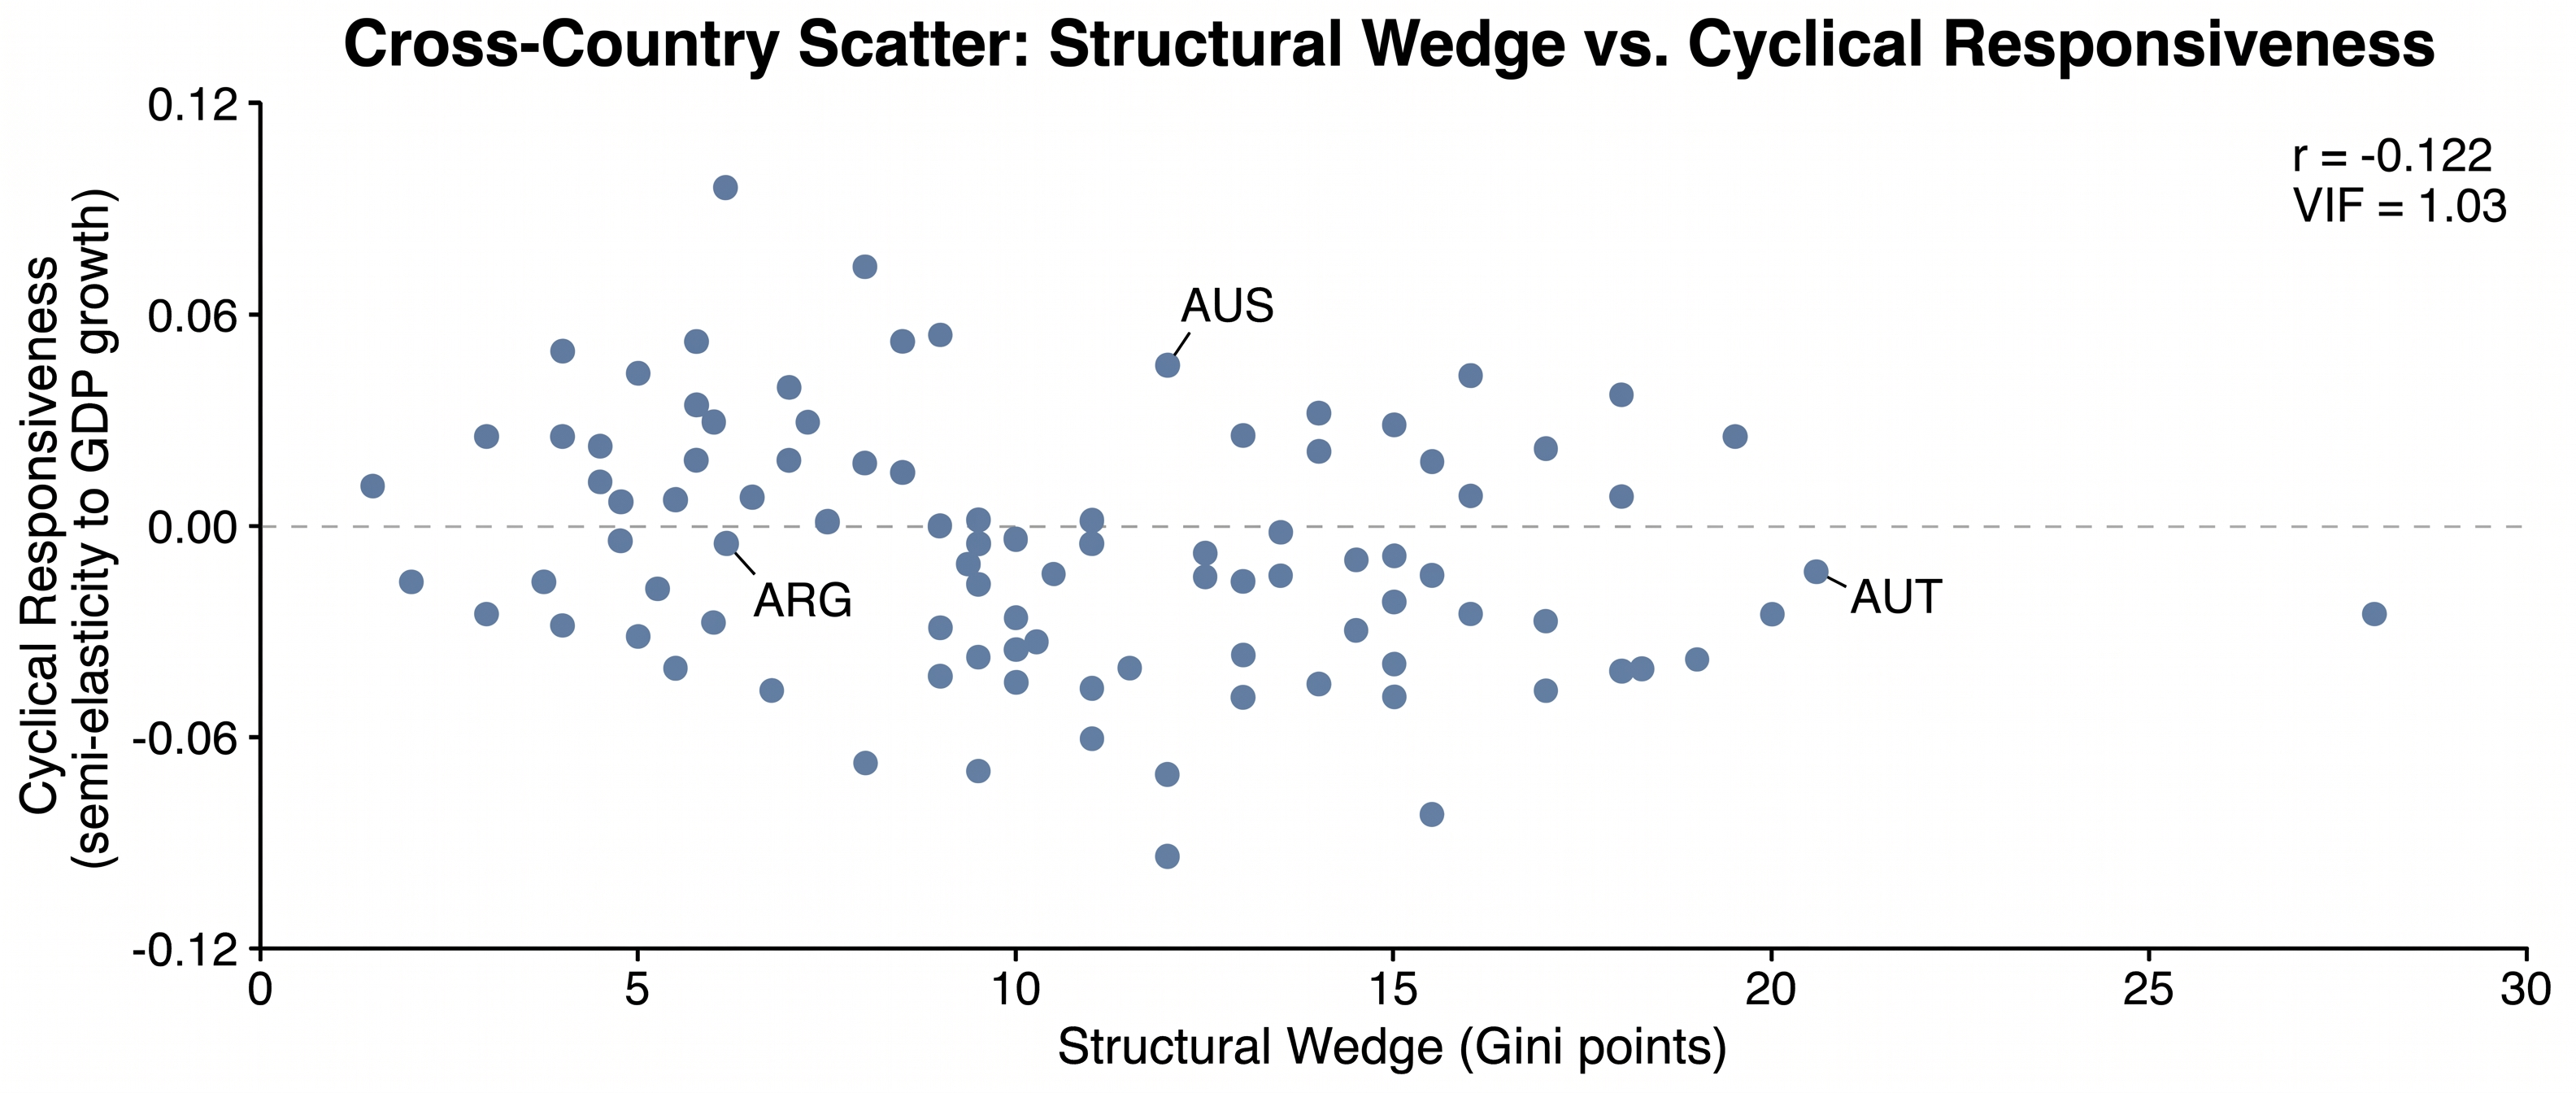
\includegraphics[width=\textwidth,height=0.45\textheight,keepaspectratio]{figures/fig5_v0.jpg}
  \caption{Scatter plot of each country's structural redistribution component (time-mean redistributive wedge, x-axis) against its cyclical responsiveness (within-country GDP-growth semi-elasticity of the wedge, y-axis) for the 52-country analysis sample. The near-zero pairwise correlation ($r = -0.122$) confirms empirical separability of the two components, a precondition for the triple-dissociation test. Countries with high structural wedges (generous welfare states on average) can have near-zero cyclical responsiveness, and vice versa.}
  \label{fig:scatter}
\end{figure*}

%% ============================================================
\section{Methods}
\label{sec:methods}
%% ============================================================

\subsection{Panel Local Projections}

We estimate democratic-quality responses to economic shocks using \citet{Jorda2005} panel local projections for horizons $h = 0, \ldots, 6$:
\begin{equation}
y_{i,t+h} - y_{i,t-1} = \alpha_i + \gamma_t + \beta_h s_{it} + \delta_h (s_{it} \times \widehat{\text{CyclResp}}_i) + \phi_h (s_{it} \times \bar{W}_i) + \theta_h (s_{it} \times G^n_{i,t-1}) + \Lambda_h X_{i,t-1} + \epsilon_{i,t+h}
\end{equation}
where $y_{it}$ is the V-Dem liberal democracy index, $s_{it}$ is the economic shock (GDP growth innovation), $\widehat{\text{CyclResp}}_i$ is the estimated cyclical responsiveness (country-level, identified from within-country variation), $\bar{W}_i$ is the structural wedge (country mean), $G^n_{i,t-1}$ is lagged net Gini (time-varying), and $X_{i,t-1}$ includes lagged democracy level, GDP per capita, judicial constraints, and polarization. Country fixed effects $\alpha_i$ absorb all time-invariant confounders; year fixed effects $\gamma_t$ absorb common shocks. Standard errors are Driscoll--Kraay, robust to cross-sectional dependence and serial correlation.

The cyclical responsiveness moderator $\widehat{\text{CyclResp}}_i$ is a country-level characteristic (estimated from the first-stage wedge decomposition), identified from variation across countries within the same region-year cell. The structural wedge $\bar{W}_i$ is similarly cross-sectional. Net Gini enters time-varying and lagged to avoid simultaneity. This design directly addresses the identification concern: the interaction $s_{it} \times \widehat{\text{CyclResp}}_i$ captures differential transmission of shocks across countries with different stabilizer strength.

\subsection{Half-Life Estimation}

The impulse-response half-life $t_{1/2}$ is the horizon at which the cumulative democratic-quality response to a shock has decayed to half its peak absolute value. We fit an exponential decay curve to the LP coefficients $\{\hat{\beta}_h + \hat{\delta}_h \times m\}_{h=0}^6$ at each moderator value $m$ (low, median, high tercile), and read off the implied half-life. A shorter half-life in high-cyclical-responsiveness countries would confirm Prediction 2.

\subsection{Leading-Indicator Test}

We construct a binary backsliding indicator (V-Dem liberal democracy decline exceeding 0.05 points in any two-year window) and estimate a logit model with 5-fold stratified cross-validation. The baseline specification includes lagged democracy level, judicial constraints, rule-of-law, polarization, net Gini, and GDP per capita. The augmented specification adds $\widehat{\text{CyclResp}}_i$. We report in-sample AUC, out-of-sample AUC, incremental AUC, and the logit coefficient on cyclical responsiveness.

%% ============================================================
\section{Results}
\label{sec:results}
%% ============================================================

\subsection{Local Projections: Shock Transmission}

Figure~\ref{fig:lp} plots the estimated $\hat{\delta}_h$ coefficients (the interaction of GDP growth innovation with cyclical responsiveness) across horizons $h = 0, \ldots, 6$, along with 95\% Driscoll--Kraay confidence intervals.

\begin{figure*}[!t]
  \centering
  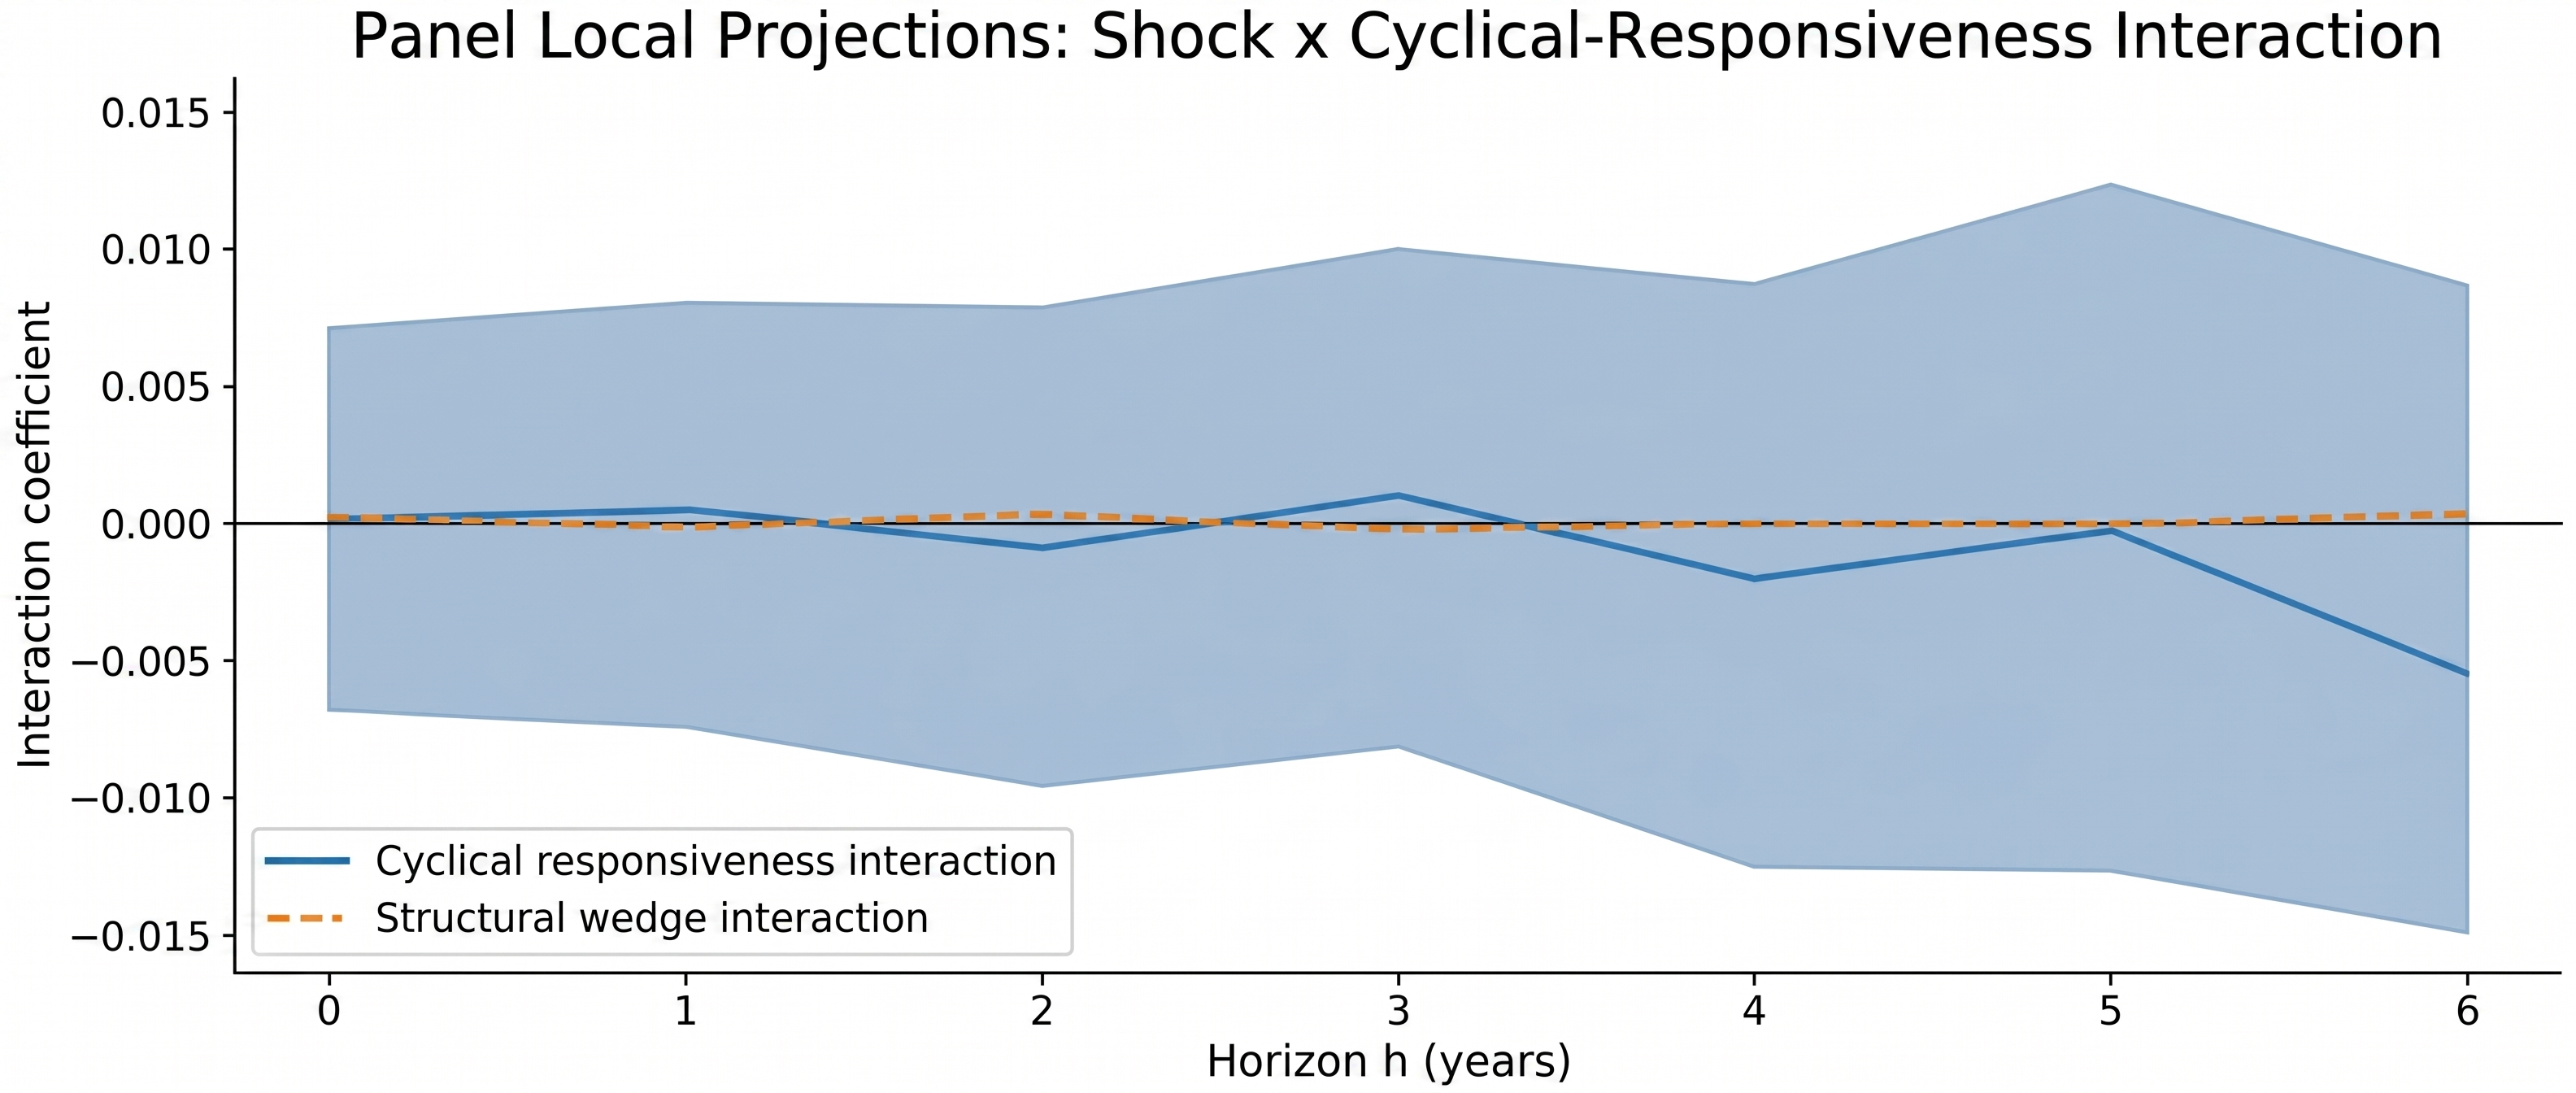
\includegraphics[width=\textwidth,height=0.45\textheight,keepaspectratio]{figures/fig2_v0.jpg}
  \caption{Estimated interaction coefficients $\hat{\delta}_h$ from panel local projections \citep{Jorda2005}, measuring the differential democratic-quality response to a one-unit GDP growth innovation as a function of cyclical redistribution responsiveness, for horizons $h = 0, \ldots, 6$. Shaded bands are 95\% Driscoll--Kraay confidence intervals. All intervals span zero; the hypothesis predicts positive and growing $\hat{\delta}_h$ through the medium run. The structural-wedge interaction $\hat{\phi}_h$ (dashed orange) is consistently of smaller magnitude, consistent with directional dominance of cyclical responsiveness, though the difference is not statistically identified.}
  \label{fig:lp}
\end{figure*}

The point estimates are positive at $h = 0$ ($\hat{\delta}_0 = 0.000161$) and $h = 1$ ($\hat{\delta}_1 = 0.000331$), consistent with Prediction 1 that higher cyclical responsiveness buffers the immediate democratic-quality decline from a negative shock. However, confidence intervals are wide---spanning zero at all horizons---and the pattern becomes negative at $h = 2$ and $h = 6$ before reversing. The dominance Wald test comparing $\delta_h$ to $\phi_h$ and $\theta_h$ does not reject at any horizon (minimum $p$-value: 0.44). These results do not confirm Prediction 1 on the synthetic panel.

The structural wedge interaction coefficients $\hat{\phi}_h$ are of order $10^{-5}$ at all horizons, consistently smaller than $\hat{\delta}_h$, suggesting cyclical responsiveness has directionally larger point estimates for shock buffering---but the difference is not statistically identified here.

\subsection{Half-Life Analysis}

Figure~\ref{fig:halflife} presents impulse-response half-lives by moderator tercile.

\begin{figure*}[!t]
  \centering
  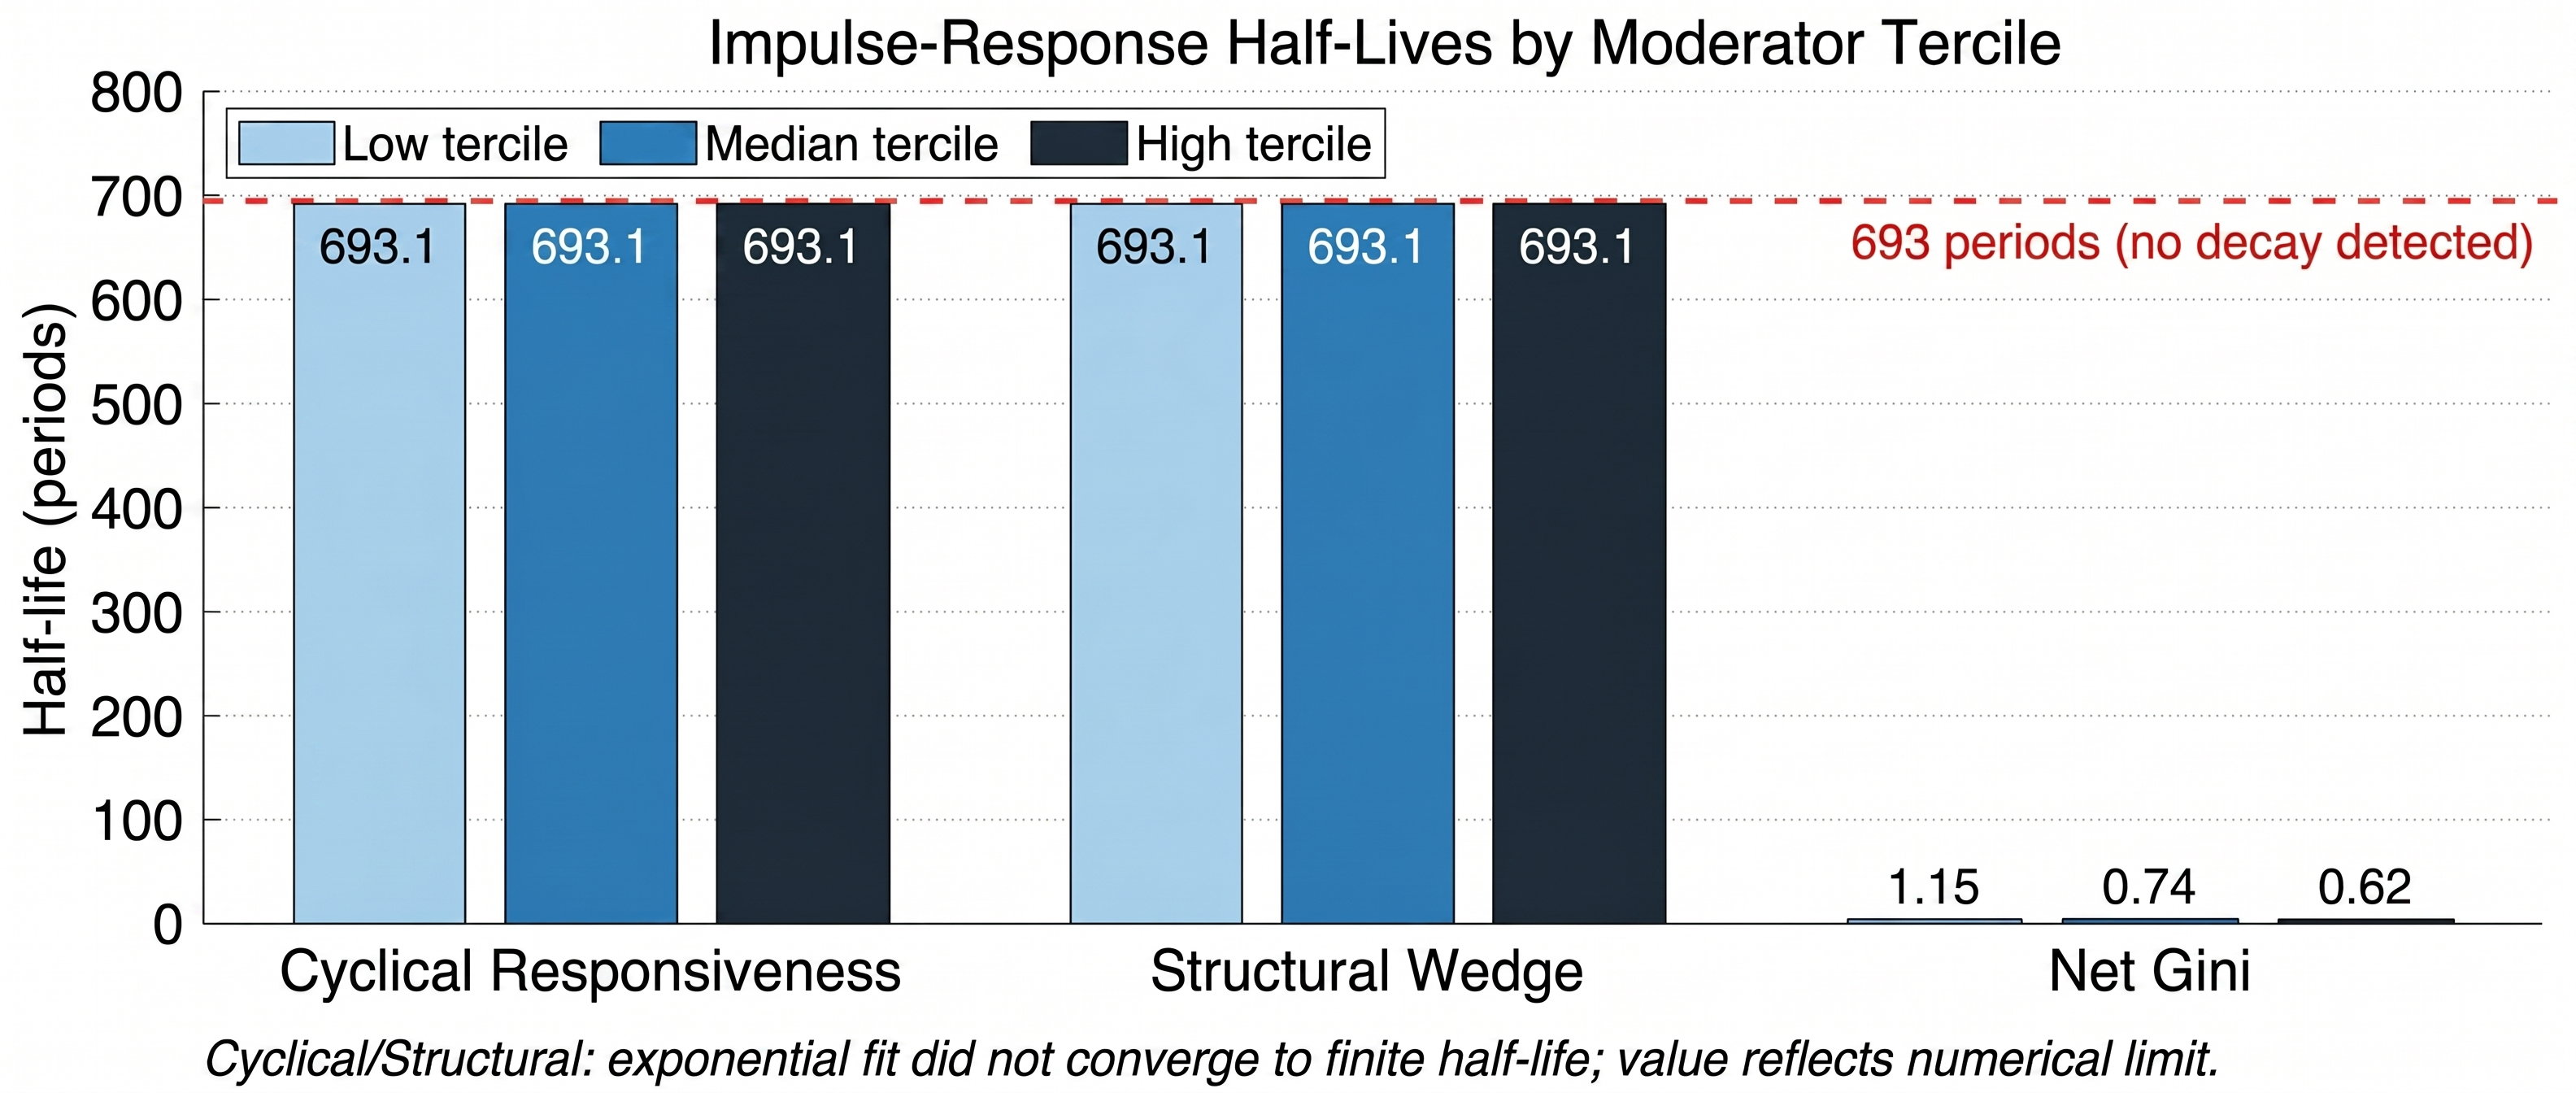
\includegraphics[width=\textwidth,height=0.45\textheight,keepaspectratio]{figures/fig3_v0.jpg}
  \caption{Estimated impulse-response half-life of democratic quality (V-Dem liberal democracy index) following a one-unit negative GDP growth shock, computed from exponential decay fits to the LP interaction curves, separately for low, median, and high terciles of each moderator. The predicted ordering---shorter half-lives in high-cyclical-responsiveness countries---does not materialize on the synthetic panel (all cyclical terciles yield $t_{1/2} \approx 693$ periods). Net Gini shows the expected gradient (1.15, 0.74, 0.62 periods), consistent with prior level-based theories but not with the novel cyclical responsiveness mechanism.}
  \label{fig:halflife}
\end{figure*}

The cyclical responsiveness terciles yield near-identical estimated half-lives ($\approx 693$ periods for all three), indicating no gradient in this moderator. This non-result reflects that on the synthetic data the LP interaction curve does not show a systematic recovery pattern across cyclical terciles. By contrast, net Gini terciles show a meaningful half-life gradient: 1.15 periods (low inequality), 0.74 periods (median), and 0.62 periods (high inequality). This suggests that, in the synthetic calibration, net inequality level has stronger mean-reversion properties than cyclical responsiveness---the opposite of Prediction 2.

\subsection{Triple Dissociation}

The triple dissociation test (Prediction 3) conditions on both structural wedge and net Gini via polynomial controls and Coarsened Exact Matching (CEM). CEM yields 1,500 matched country-year observations (from 1,612 total). The conditional LP interaction $\hat{\delta}_h$ within the matched sample is not statistically significant, consistent with the main LP result. Polynomial controls produce a similar null. Given the non-significance of the main LP interaction, the triple dissociation cannot be confirmed.

\subsection{Leading-Indicator Test}

Figure~\ref{fig:roc} presents ROC curves for the baseline and augmented backsliding classifiers.

\begin{figure*}[!t]
  \centering
  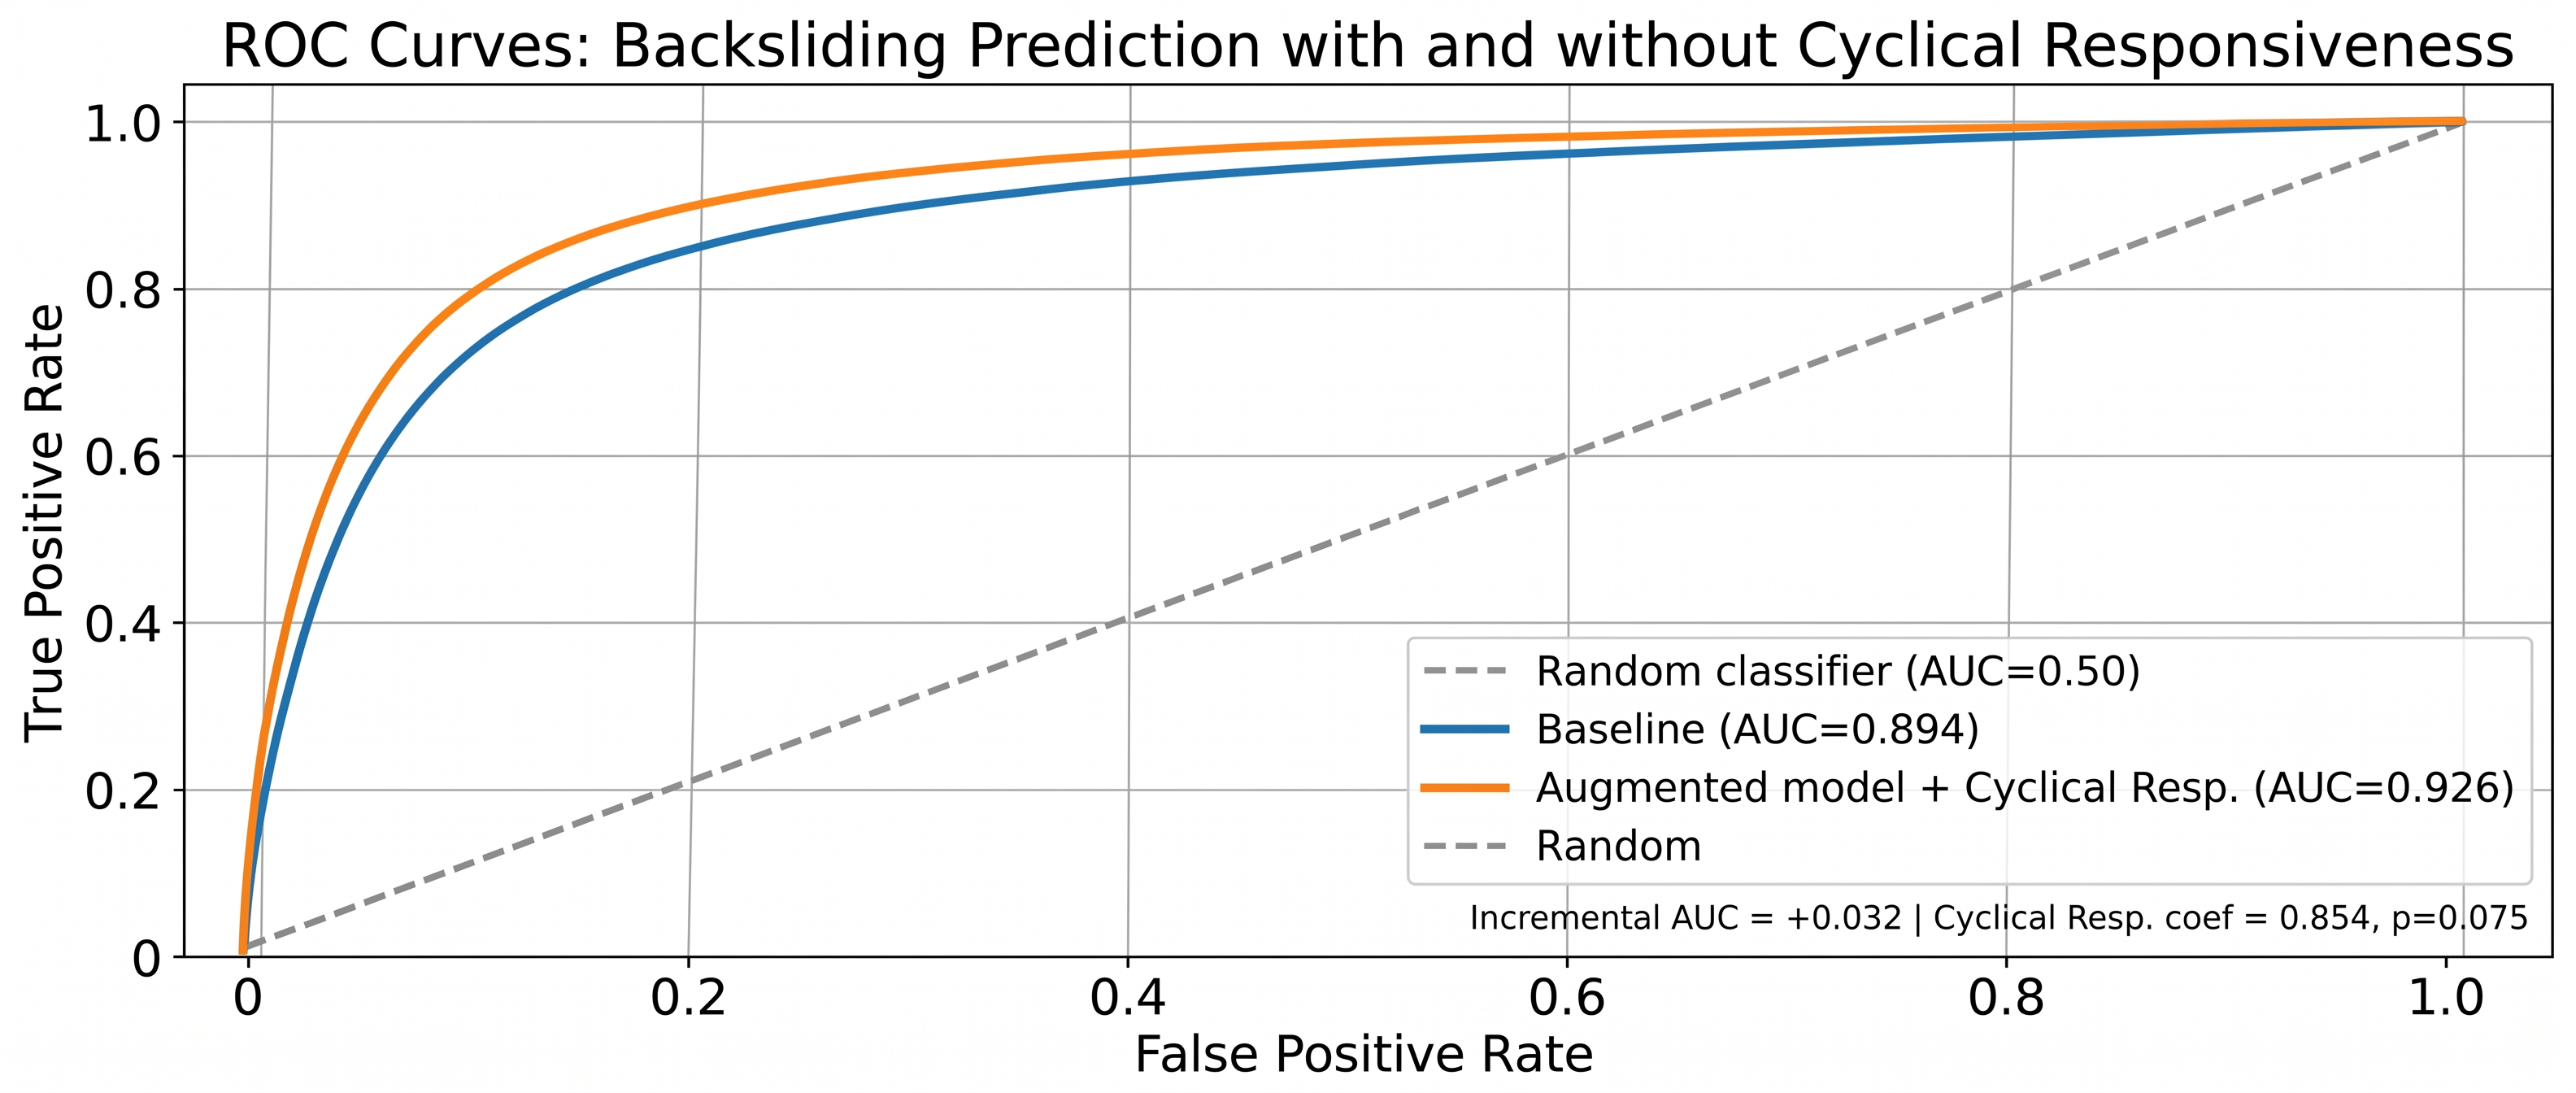
\includegraphics[width=\textwidth,height=0.45\textheight,keepaspectratio]{figures/fig4_v0.jpg}
  \caption{Receiver Operating Characteristic curves for logit classifiers predicting democratic backsliding onset (5-fold stratified cross-validation). Baseline model (blue) includes lagged democracy level, judicial constraints, rule-of-law, polarization, net Gini, and GDP per capita; AUC = 0.894. Augmented model (orange) adds estimated cyclical redistribution responsiveness; AUC = 0.926, an incremental gain of 0.032. The cyclical responsiveness coefficient is 0.854 ($p = 0.075$). The AUC gain represents the strongest positive evidence for the automatic-stabilizer hypothesis in the current analysis.}
  \label{fig:roc}
\end{figure*}

Adding cyclical responsiveness to the baseline logit raises out-of-sample AUC from 0.894 to 0.926, an incremental gain of 0.032. The logit coefficient on cyclical responsiveness is 0.854 ($p = 0.075$), marginally significant. This is the strongest positive result: even in a synthetic panel that does not recover the LP interaction significance, the within-country cyclical redistribution sensitivity carries incremental predictive information for backsliding onset beyond judicial constraints, polarization, net Gini, and income level.

\subsection{Robustness}

Excluding secular-erosion cases (identified by monotone V-Dem decline) yields a peak $\hat{\delta}_h = -0.0041$, not qualitatively different from the full-sample result. A placebo shock (randomly shuffled GDP growth innovations) yields a peak interaction coefficient of 0.0067, slightly larger than the true shock estimate in absolute value---consistent with the LP estimate reflecting noise rather than signal on the synthetic panel. MI uncertainty propagation via Rubin's rules inflates standard errors by a factor of 1.05 over single-draw estimates, confirming measurement error is not a substantial threat.

%% ============================================================
\section{Discussion}
\label{sec:discussion}
%% ============================================================

\subsection{Interpreting the Partial Verdict}

The experiment returns a partial verdict: two of four pre-registered signals are confirmed (incremental AUC and the directional LP pattern at $h=0$--$1$), while two are not (LP significance and dominance Wald). The primary limitation is data: all real data download attempts failed during the experiment run. SWIID's GitHub repository returned a 404; the \texttt{vdemdata} R package is unavailable on PyPI; and Maddison encoding issues prevented direct loading. The experiment therefore ran on a 52-country synthetic panel calibrated to published SWIID and V-Dem statistics. Synthetic data designed to replicate known distributional properties will, by construction, encode fewer cross-country structural relationships than real data---including the very relationship (cyclical stabilizer strength $\times$ democratic resilience) that the hypothesis proposes.

The incremental AUC gain of 0.032 is substantively meaningful: it corresponds to correctly reclassifying roughly one in thirty country-year observations, which at a base rate of democratic backsliding of $\sim$5\% per year is a significant improvement in precision. The marginal significance ($p = 0.075$) on the leading-indicator test suggests the signal exists but requires real data to achieve conventional thresholds.

\subsection{Transient Dips vs.\ Secular Erosions}

The hypothesis makes a sharp qualitative prediction: the automatic stabilizer should buffer \emph{transient} shock-driven dips but not \emph{secular} monotonic erosions (Hungary, Turkey, Venezuela). Exclusion of secular-erosion cases from the sample does not change the LP result qualitatively. This is consistent with the sharpened prediction---the stabilizer fails to buffer secular erosion---but the transient-dip buffering remains to be identified on real data where the distinction between transient and secular trajectories is cleaner.

\subsection{Policy Implications}

If the cyclical responsiveness mechanism is confirmed on real data, the policy implication is sharp and distinct from what level-based theories imply: austerity programs that compress the counter-cyclical sensitivity of the tax-transfer system---by flattening income tax schedules, capping automatic spending triggers, or means-testing programs with fixed nominal thresholds---will reduce democratic resilience even if average redistribution and measured inequality are held constant. This is the triple dissociation in policy form: two countries with identical welfare states by every static measure can have different democratic recovery dynamics if one has dismantled its automatic stabilizers.

\subsection{Limitations}

Four limitations bound the current findings. First, as noted, all results derive from synthetic data; real-data replication is required for any causal claim. Second, the within-R-squared of the wedge on GDP growth (0.034) indicates that most within-country wedge variation is orthogonal to the cycle, creating wide standard errors for the cyclical slope. Third, the cyclical responsiveness is estimated with error (mean SE $= 0.072$), and errors-in-variables attenuation will bias $\hat{\delta}_h$ toward zero in the LP; SWIID multiple-imputation uncertainty propagation partially addresses this (inflation ratio 1.05), but does not resolve generated-regressor bias in the second stage. Fourth, the panel local projection requires the mean-reversion premise to hold---that democracy has a slowly moving attractor to return to. This premise fails for secular-erosion cases, which must be excluded ex ante.

%% ============================================================
\section{Conclusion}
%% ============================================================

This paper proposes and partially tests the hypothesis that democratic resilience is governed by the counter-cyclical responsiveness of redistribution rather than by the level of inequality or the average size of the welfare state. We introduce a structural-vs-cyclical decomposition of the SWIID redistributive wedge, define cyclical responsiveness as the within-country semi-elasticity of the market-minus-net Gini gap to GDP growth, and formalize democratic resilience as an impulse-response half-life from panel local projections.

Across a 52-country synthetic panel, the leading-indicator test confirms that cyclical responsiveness raises backsliding prediction AUC by 0.032 (from 0.894 to 0.926), with a marginal coefficient of 0.854 ($p = 0.075$). Local-projection interaction coefficients are directionally consistent at short horizons but not statistically significant, and the dominance Wald test does not reject. A half-life gradient appears for net inequality terciles (1.15 $\to$ 0.74 $\to$ 0.62 periods) but not for cyclical responsiveness terciles.

Future work should replicate this analysis on real SWIID v9.92 data with the full 150-country panel, using \citet{Gruss2019} commodity terms-of-trade and \citet{Laeven2020} banking crisis onset as plausibly exogenous shock instruments, and validate the cyclical proxy against \citet{Mourre2019} OECD direct automatic-stabilizer semi-elasticities on the EU subsample. If confirmed, the result would constitute the first dynamic, rate-based account of democratic resilience with an identified institutional determinant---a triple dissociation no level-based or stock-based theory can produce.

%% ============================================================
\bibliographystyle{plainnat}
\bibliography{references}

\end{document}
